\chapter{Advanced Learning}
Nei capitoli precedenti (\ref{sec:stocastic_gradient_descent}) abbiamo visto come minimizzare una certa funzione di loss usando il gradiente
\begin{equation}
	\vec{w}^{k+1} = \vec{w}^k - \eta \nabla_{\vec{w}} E(\vec{w})
\end{equation}
Ci domandiamo ora come rendere efficiente il training, sia modificando i parametri dell'equazione appena mostrata sia modificando proprio la strategia di learning.

\section{Learning rate}
La scelta del learning rate corretto è fondamentale per avere una rete che converga al minimo globale dell'errore, infatti se abbiamo learning rate
\begin{multicols}{3}
	\begin{itemize}
		\item troppo piccolo finiremo incastrati in minimi locali;
		\item corretto riusciamo a individuare il minimo globale;
		\item troppo grande la rete non converge a un minimo.
	\end{itemize}
\end{multicols}
\begin{center}
	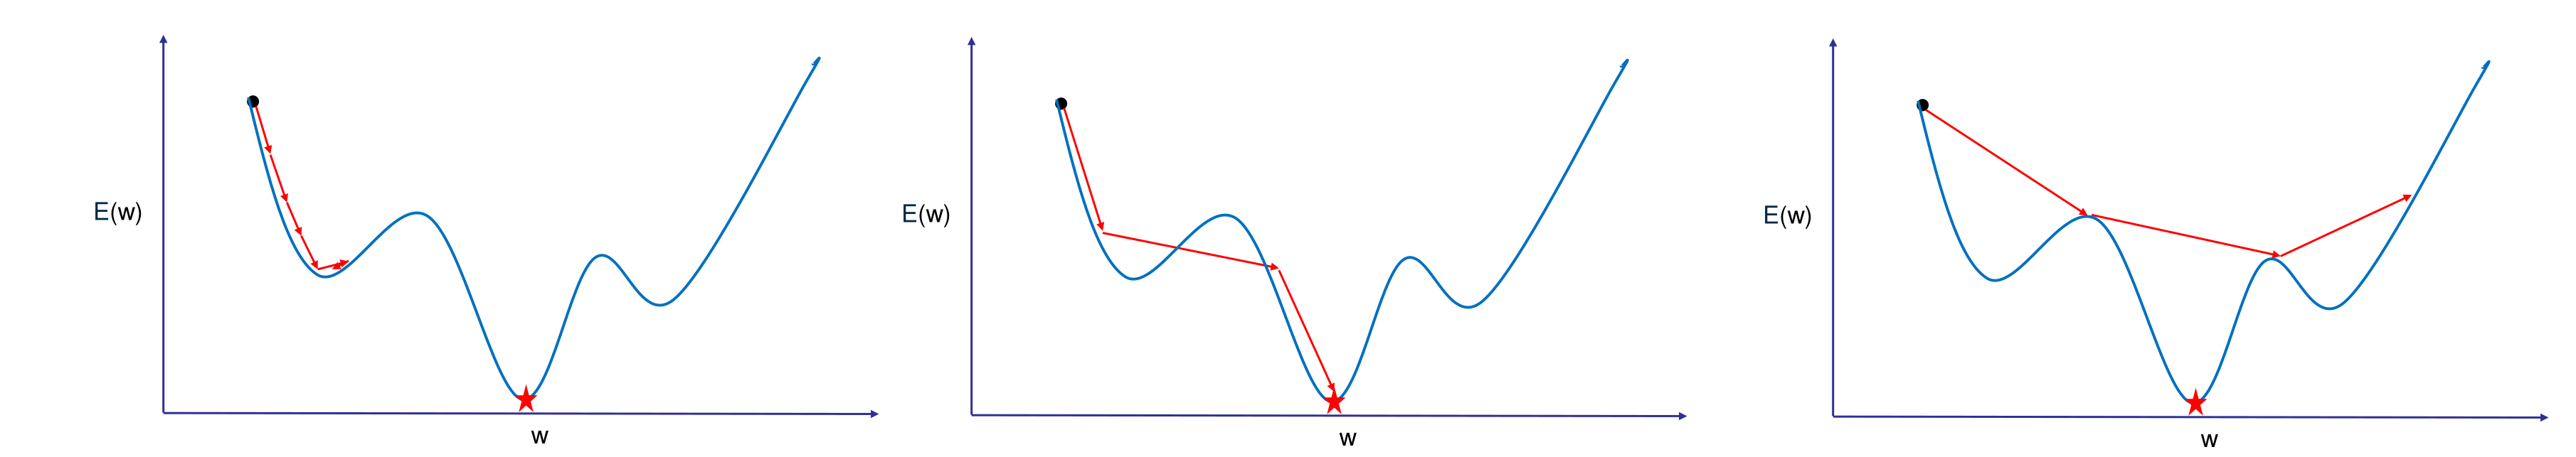
\includegraphics[width=\linewidth]{Picture/Learning_Rate}
\end{center}

L'idea è che all'inizio dell'allenamento la rete si strovi a grande distanza dal minimo globale, man mano che vengono appresi i pesi ci si avvicina e gli step verso il minimo si fanno più piccoli. Per sfruttare questa idea si può modificare il learning rate durante l'apprendimento.

\subsection{Decadimento del learning rate}
Per modificare il learning rate possiamo seguire diverse politiche, in questo paragrafo ci concentriamo sulle più semplici che sono monotone decrescenti, ma esistono alti modi di far variare il learnin rate che non sono monotoni e possono riuscire a non incastrarsi in minimi locali.
\subsubsection{Step decay}
Dopo in certo numero di iterazioni (\textbf{epoche}) il learning rate viene moltiplicato per un valore $<1$ in modo da rendere il suo grafico un decadimento esponenziale a gradini. Le epoche in cui avviene la riduzione del learning rate sono dette \textbf{milestones}. Formalmente a ogni milestones il learning rate viene aggiornato in questo modo:
\begin{equation}
	\eta = \eta_0 \cdot e^{-kt}
\end{equation}
dove $\eta_0$ è il learning rate iniziale, $k$ è il numero della milestones e $t$ è un parametro.
\subsubsection{Time decay}
Dopo ogni epoca il learning rate iniziale viene diviso per  il numero di epoche opportunamente pesato. In questo caso il grafico del learning rate è un ramo di iperbole. Formalmente
\begin{equation}
	\eta = \frac{\eta_0}{1 + k\cdot t}
\end{equation}
dove $\eta_0$ è il learning rate iniziale, $k$ è il numero dell'epoca attuale e $t$ è un parametro.
\subsubsection{Exponential decay}
Come lo step decay, ma l'aggiornamento viene fatto dopo ogni epoca. Formalmente
\begin{equation}
	\eta = \eta_0 \cdot e^{-kt}
\end{equation}
dove $\eta_0$ è il learning rate iniziale, $k$ è il numero dell'epoca attuale e $t$ è un parametro.
\newpage
\section{Stocastic gradient descent}
\begin{wrapfigure}{r}{.5\linewidth}
	\vspace{-.25cm}
	\centering
	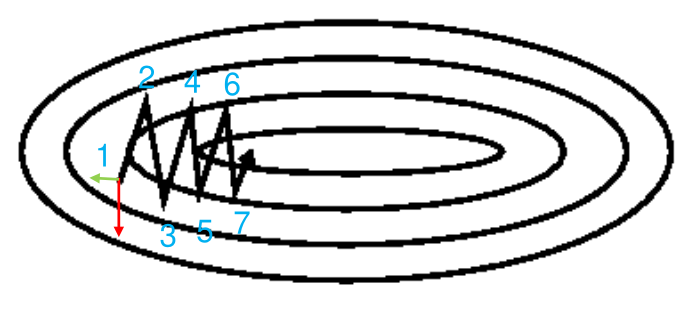
\includegraphics[width=\linewidth]{Picture/SGD}
\end{wrapfigure}
Lo stocastic gradient descent SGD presenta dei problemi quando incontriamo una valle, infatti se osserviamo la situazione dell'immagine è facile convincersi che mentre le frecce verdi rimarranno costanti e orientate verso il minimo le frecce rosse invertono il loro segno ogni volta, questo provoca una discesa a zigzag dell'errore (poco efficiente). Quando si verifica lo zigzag diciamo che il \textbf{gradiente è rumoroso} in quella dimensione, dato che cambia tutte le volte di segno.

\subsection{Aggiunta della quantità di moto}
Per limitare il rumore di alcune componenti del gradiente si può ricorrere a delle similitudini con la fisica. Una pallina lanciata nel punto 1 farà poche oscillazioni ampie, per poi accelerare maggiormente verso il minimo. Esattamente come mostrato nell'immagine.

\begin{wrapfigure}{l}{.5\linewidth}
	\vspace{-.25cm}
	\centering
	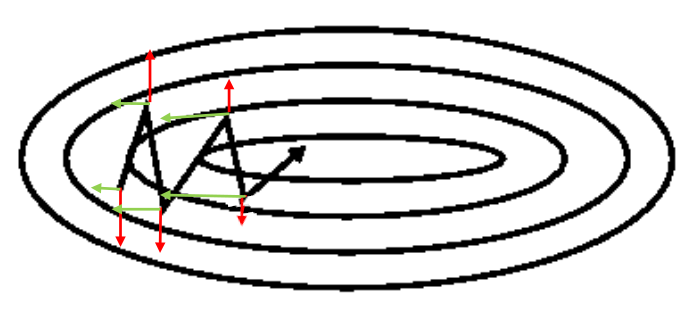
\includegraphics[width=\linewidth]{Picture/SGD_Momentum}
\end{wrapfigure}
Per replicare questo comportamento si aggiunge una sorta di conservazione della quantità di moto (in inglese momentum) che si oppone all'oscillare del segno delle componenti rumorose del gradiente. La componente inerziale che aggiungiamo al gradiente è semplicemente il gradiente calcolato all'iterazione precedente. Formalmente all'iterazione $k+1$ avremo:
\begin{equation}
	\vec{w}^{k+1} = \vec{w}^k - \eta (\nabla_{\vec{w}} E(\vec{w}^k) + \nabla_{\vec{w}} E(\vec{w}^k))
\end{equation}

\subsection{Tecniche avanzate di discesa del gradiente}
Sono stati ingegnerizzati moltissimi altri ottimizzatori ciascuno che punta a risolvere le criticità dei precedenti. La maggior parte di questi è già implementata nei framework per l'AI, Pythorch offre:
\begin{multicols}{4}
	\begin{itemize}
		\item Adadelta
		\item Adagrad
		\item Adam
		\item ASDG
		\item LBFGS
		\item Rprop
		\item SDG
		\item Ecc\dots
	\end{itemize}
\end{multicols}

\section{Batch Training}
In uno scenario ideale tutti i campioni del set di training ci portano verso il minimo globale, nella realtà pero i dati del set possono essere  effetti da errore, questo fa si che campione per campione il minimo si trovi in posizione diversa e questo porta a oscillare intorno al minimo piuttosto che a raggiungerlo.

Per mitigare l'effetto degli errori e del rumore nei campioni di training si ricorre a tecniche statistiche.

\subsection{Minibatch}
Al posto che addestrare la rete campione per campione si divide il set di training in minibatch di $m$ campioni. E si usano i risultati dell'addestramento sull'intero mini batch per aggiornare i pesi della rete.
\vspace{.5cm}
\begin{algorithmic}
	\Function{MiniBatchTraining}{}
		\ForAll {minibatch $b$ in $trainingSet$}
			\State $\vec{G} \gets 0$ \Comment{init. accumulatore gradiente}
			\ForAll{sample $x$ in $b$}
				\State $y \gets$ \Call{NetInference}{x} \Comment{risultato della rete}
				\State $E \gets$ \Call{LossFunction}{y}
				\State $\vec{g} \gets \nabla_{\vec{w}}E(\vec{w})$ \Comment{Calcolo gradiente}
				\State $\vec{G} \gets \vec{G} + \vec{g}$ \Comment{Accumulo gradienti}
			\EndFor
			\State $\vec{w}^{b + 1} \gets \vec{b} + \eta \frac{1}{m} \vec{G}$ \Comment{Aggiorno pesi con la media del gradiente}
		\EndFor
	\EndFunction    
\end{algorithmic}

\begin{wrapfigure}[5]{r}{.3\linewidth}
	\vspace{-1.2cm}
	\centering
	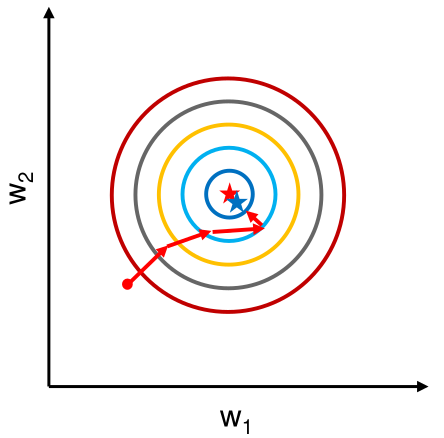
\includegraphics[width=.9\linewidth]{Picture/Batch_Training1}
	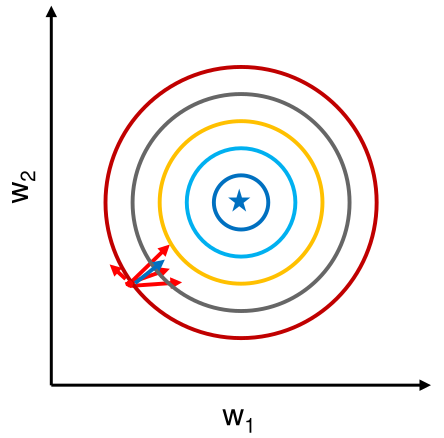
\includegraphics[width=.9\linewidth]{Picture/Batch_Training2}
\end{wrapfigure}
\vspace{.5cm}
L'immagine mostra le differenze tra un addestramento sample per sample e uno fatto con i minibatch. Questo approccio
\begin{itemize}
	\item permette convergenza più rapida dovuta ai minori errori
	\item è la chiave delle architetture profonde
	\item rendere computazionalmente efficiente il training
	\item permette di mischiare immagini di classi diverse in un solo aggiornamento dei pesi
\end{itemize}

\section{Overfitting}
Nel capitolo introduttivo (\ref{sec:regularization}) abbiamo già parlato di come la regolarizzazione possa prevenire l'overfitting, vediamo ora altre tecniche che di solito vengono usate in aggiunta alla regolarizzazione.

\subsection{Data Augmentation}
Dato che le reti neurali hanno bisogno di moltissimi esempi per l'addestramento quelli nel set di training possono non essere sufficienti. Si ricorre allora alla data augmentation che consiste nel sintetizzare nuove immagini a partire da quelle presenti nel set.

Per sintetizzare nuove immagini si può ricorrere a diverse trasformazioni, modificando ad esempio:

\begin{wrapfigure}[5]{r}{.6\linewidth}
	\vspace{-.7cm}
	\centering
	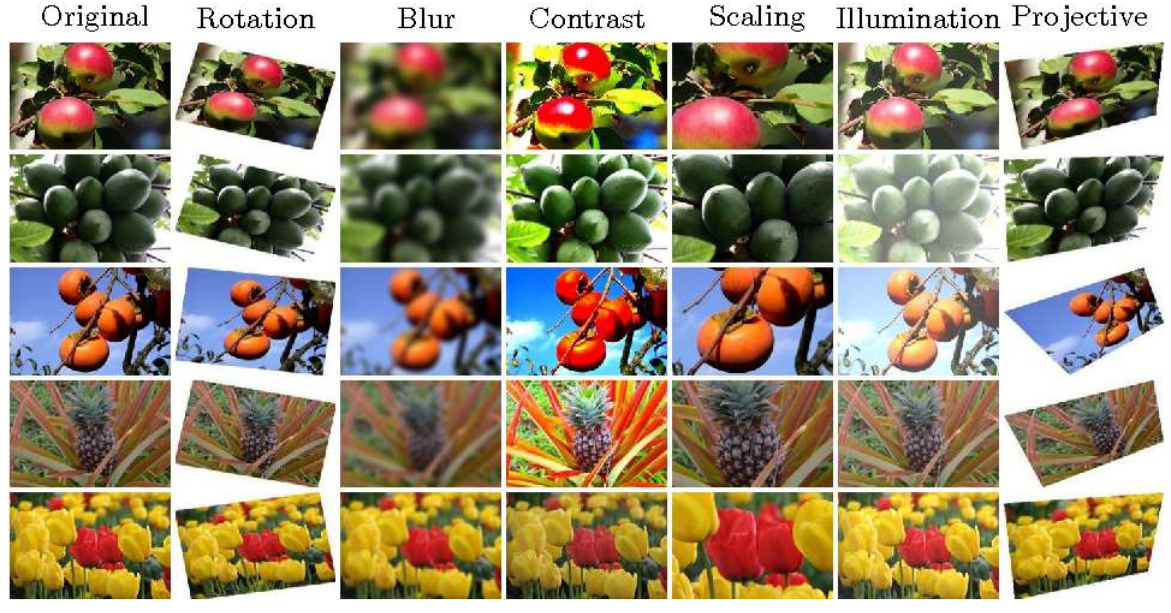
\includegraphics[width=.9\linewidth]{Picture/Data_Augmentation}
\end{wrapfigure}
\ 
\vspace{-.5cm}
\begin{multicols}{2}
	\begin{itemize}
		\item Scala
		\item Rotazione
		\item Traslazione
		\item Blur
		\item Contrasto
		\item Luminosità
		\item Proiezione
		\item Ecc\dots
	\end{itemize}
\end{multicols}
\vspace{.5cm}
L'immagine mostra esempi di data augmentation relativi a un set di immagini per il riconoscimento dei frutti. Ovviamente non tutte le trasformazioni sono ammissibili, ad esempio se dobbiamo riconoscere del testo non possiamo ruotare di $180^{\circ}$ i caratteri.

Grazie alla data augmentation possiamo aunentare la diversità intra-classe dei dati, si è visto sperimentalmente che questo approccio porta a vantaggi notevoli, ad esempio la LeNet300 che abbiamo presentato prima (\ref{sec:LeNet300}) dopo la data augmentation passa da un tasso di errore del $3.05\%$ a uno del $2.45\%$

\subsection{Committees of Neural Networks}
L'overfitting è spesso causato dal fatto che ci sono troppi pochi campioni perchè una rete complessa possa apprendere la generalità del problema. Questo approccio quindi consiste nel dividere la rete complessa in tante reti più semplici e unire i risultati degli output di ciascuna per prendere la decisione finale. In questo modo si riduce il numero di parametri di ciascuna rete e si previene l'overfitting. 

È importantissimo in questo caso inizializzare i pesi delle sotto-reti in modo attento, non vogliamo avere tante copie di una rete, ma molte reti diverse ciascuna cche ha appreso in modo diverso come risolvere il problema.

In base alla tipologia del problema si potranno unire i risultati in modo diverso:
\begin{itemize}
	\item \textbf{Classificazione}: il risultato definitivo sarà quello più votato dalle sotto-reti;
	\item \textbf{Regressione}: il risultato può essere ottenuto facendo la media dei risultati forniti.
\end{itemize}

\subsection{Dropout}
Per rendere più snella la rete un fase di training si possono interrompere alcuni collegamenti nei vari layer, i neuroni alimentati da questi collegamenti resteranno spenti. 

\begin{wrapfigure}{r}{.4\linewidth}
	\vspace{-.7cm}
	\centering
	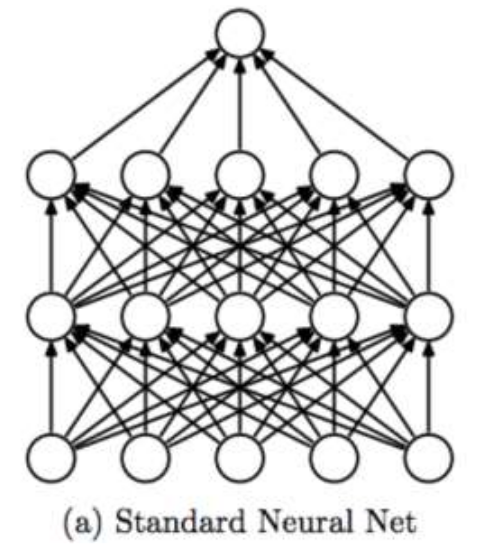
\includegraphics[width=.9\linewidth]{Picture/Dropout1}
	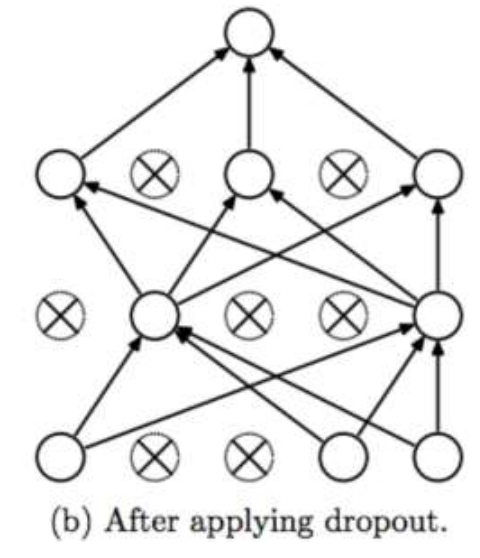
\includegraphics[width=.9\linewidth]{Picture/Dropout2}
\end{wrapfigure}
La strategia tipica è quella di scegliere un certo tasso di dropout e ogni neurone avrà quella porpbabilità di essere disattivato.

I neuroni spenti non partecipano alla creazione dell'output, né al calcolo del gradiente, inoltre i loro pesi non saranno aggiornati.

Terminato il training tutti i neuroni partecipano all'inferenza, ma l'output di ciscun neurone sarà ridotto in proporzione al tasso di dropout, per compensare l'assenza delle attivazioni durante il training.

Nell'immagine si vede un esempio di rete sottoposta a dropout. Questa tecnica funziona perché permette alla rete di distribuire l'apprendimento su tutti i neuroni e non far affidamento solo su alcuni (o su specifiche connessioni tra neuroni), è come se si addestrassero tante sotto-reti tutte diverse ad ogni iterazione; rendendo la rete più robusta a piccole variazioni nel training set e rendendo l'apprendimento più generale